\chapter{Resultados}

A continuación, vamos a plantear algunos casos de estudio para analizar en detalle el comportamiento del algoritmo. 
Para este análisis utilizaremos la estrategia Optimista - Nueva acción.

\section{Laberinto de 25 posiciones}

El primer entorno que presentamos es un laberinto de 25 posiciones. En cada posición el robot puede tener hasta 4 
acciones disponibles, las cuales son norte, sur, este y oeste. El entorno no tiene agentes externos. El objetivo de 
este caso de estudio es ver como el robot encuentra la salida en un laberinto complejo sin información previa.

\begin{figure}[H]
	\centering
		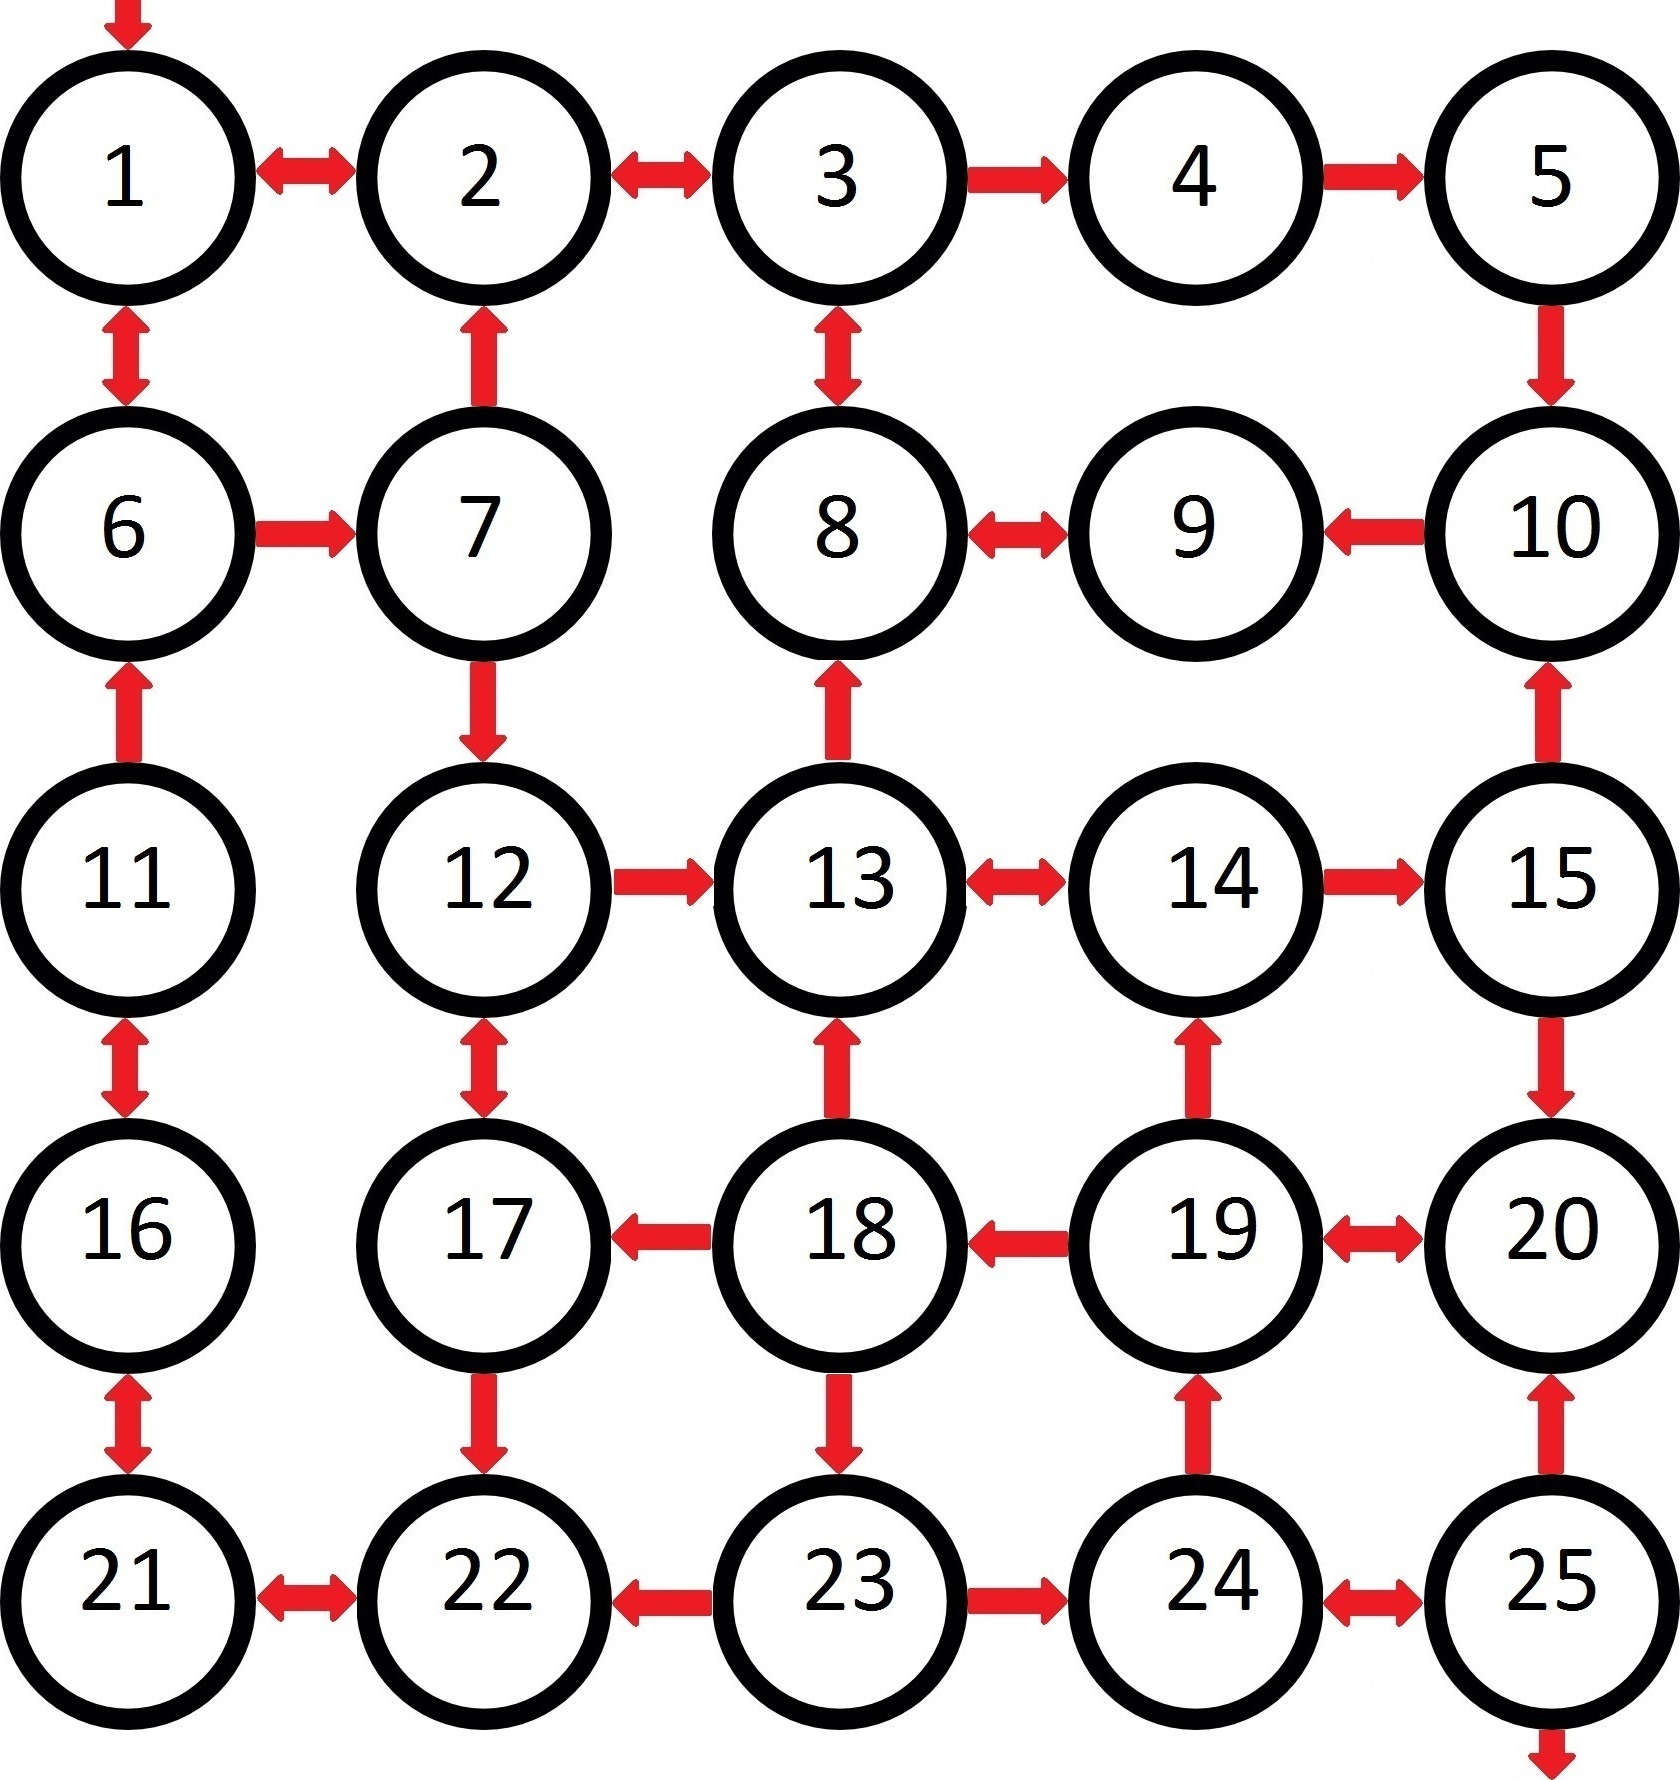
\includegraphics[width=0.9\textwidth]{Imagenes/Laberintos/25.jpg}
	\caption{Laberinto de 25 posiciones.}
	\label{fig:25}
\end{figure}

\subsection{Especificación en MTSA}

\begin{Code}[commandchars=&\[\]]
&fvtextcolor[0000A0][VIEW] = &fvtextcolor[0000A0][P01],
&fvtextcolor[0000A0][P01]  = (sur   -> &fvtextcolor[0000A0][P06] | este  -> &fvtextcolor[0000A0][P02]),
&fvtextcolor[0000A0][P02]  = (este  -> &fvtextcolor[0000A0][P03] | oeste -> &fvtextcolor[0000A0][P01]),
&fvtextcolor[0000A0][P03]  = (sur   -> &fvtextcolor[0000A0][P08] | este  -> &fvtextcolor[0000A0][P04] | oeste -> &fvtextcolor[0000A0][P02]),
&fvtextcolor[0000A0][P04]  = (este  -> &fvtextcolor[0000A0][P05]),
&fvtextcolor[0000A0][P05]  = (sur   -> &fvtextcolor[0000A0][P10]),
&fvtextcolor[0000A0][P06]  = (norte -> &fvtextcolor[0000A0][P01] | este  -> &fvtextcolor[0000A0][P07]),
&fvtextcolor[0000A0][P07]  = (norte -> &fvtextcolor[0000A0][P02] | sur   -> &fvtextcolor[0000A0][P12]),
&fvtextcolor[0000A0][P08]  = (norte -> &fvtextcolor[0000A0][P03] | este  -> &fvtextcolor[0000A0][P09]),
&fvtextcolor[0000A0][P09]  = (oeste -> &fvtextcolor[0000A0][P08]),
&fvtextcolor[0000A0][P10]  = (oeste -> &fvtextcolor[0000A0][P09]),
&fvtextcolor[0000A0][P11]  = (norte -> &fvtextcolor[0000A0][P06] | sur   -> &fvtextcolor[0000A0][P16]),
&fvtextcolor[0000A0][P12]  = (sur   -> &fvtextcolor[0000A0][P17] | este  -> &fvtextcolor[0000A0][P13]),
&fvtextcolor[0000A0][P13]  = (norte -> &fvtextcolor[0000A0][P08] | este  -> &fvtextcolor[0000A0][P14]),
&fvtextcolor[0000A0][P14]  = (este  -> &fvtextcolor[0000A0][P15] | oeste -> &fvtextcolor[0000A0][P13]),
&fvtextcolor[0000A0][P15]  = (norte -> &fvtextcolor[0000A0][P10] | sur   -> &fvtextcolor[0000A0][P20]),
&fvtextcolor[0000A0][P16]  = (norte -> &fvtextcolor[0000A0][P11] | sur   -> &fvtextcolor[0000A0][P21]),
&fvtextcolor[0000A0][P17]  = (norte -> &fvtextcolor[0000A0][P12] | sur   -> &fvtextcolor[0000A0][P22]),
&fvtextcolor[0000A0][P18]  = (norte -> &fvtextcolor[0000A0][P13] | sur   -> &fvtextcolor[0000A0][P23] | oeste -> &fvtextcolor[0000A0][P17]),
&fvtextcolor[0000A0][P19]  = (norte -> &fvtextcolor[0000A0][P14] | este  -> &fvtextcolor[0000A0][P20] | oeste -> &fvtextcolor[0000A0][P18]),
&fvtextcolor[0000A0][P20]  = (oeste -> &fvtextcolor[0000A0][&fvtextcolor[0000A0][P19]]),
&fvtextcolor[0000A0][P21]  = (norte -> &fvtextcolor[0000A0][P16] | este  -> &fvtextcolor[0000A0][P22]),
&fvtextcolor[0000A0][P22]  = (oeste -> &fvtextcolor[0000A0][P21]),
&fvtextcolor[0000A0][P23]  = (este  -> &fvtextcolor[0000A0][P24] | oeste -> &fvtextcolor[0000A0][P22]),
&fvtextcolor[0000A0][P24]  = (norte -> &fvtextcolor[0000A0][&fvtextcolor[0000A0][P19]] | este  -> &fvtextcolor[0000A0][P25]),
&fvtextcolor[0000A0][P25]  = (norte -> &fvtextcolor[0000A0][P20] | oeste -> &fvtextcolor[0000A0][P24] | salir -> &fvtextcolor[0000A0][P25]).

&fvtextcolor[0000A0][MODEL] = (norte? -> &fvtextcolor[0000A0][MODEL] | sur?   -> &fvtextcolor[0000A0][MODEL] | este? -> &fvtextcolor[0000A0][MODEL] | 
         oeste? -> &fvtextcolor[0000A0][MODEL] | salir? -> &fvtextcolor[0000A0][MODEL]).

&fvtextcolor[0000FF][set] &fvtextcolor[0000A0][Controllable_25] = {norte, sur, este, oeste, salir}
&fvtextcolor[0000FF][fluent] &fvtextcolor[0000A0][F_Salir]      = <salir, &fvtextcolor[0000A0][Controllable_25]\{salir}>
&fvtextcolor[0000FF][assert] &fvtextcolor[0000A0][A_Salir]      = &fvtextcolor[0000A0][F_Salir]

&fvtextcolor[0000FF][controllerSpec] &fvtextcolor[0000A0][GOAL_25] = {
    liveness     = {&fvtextcolor[0000A0][A_Salir]}
    controllable = {&fvtextcolor[0000A0][Controllable_25]}
}

&fvtextcolor[0000FF][exploration] &fvtextcolor[0000A0][M25] = {
    environment = {&fvtextcolor[0000A0][VIEW]},
    model       = {&fvtextcolor[0000A0][MODEL]},
    goal        = {&fvtextcolor[0000A0][GOAL_25]}
}
\end{Code}

\subsection{Análisis preliminar}

El robot logra salir del laberinto en 116 pasos, pasando en promedio 4.64 veces por cada posición. 
Podemos observar a simple vista que las posiciones más visitadas forman parte del camino hacia la salida.

\begin{figure}[H]
	\centering
		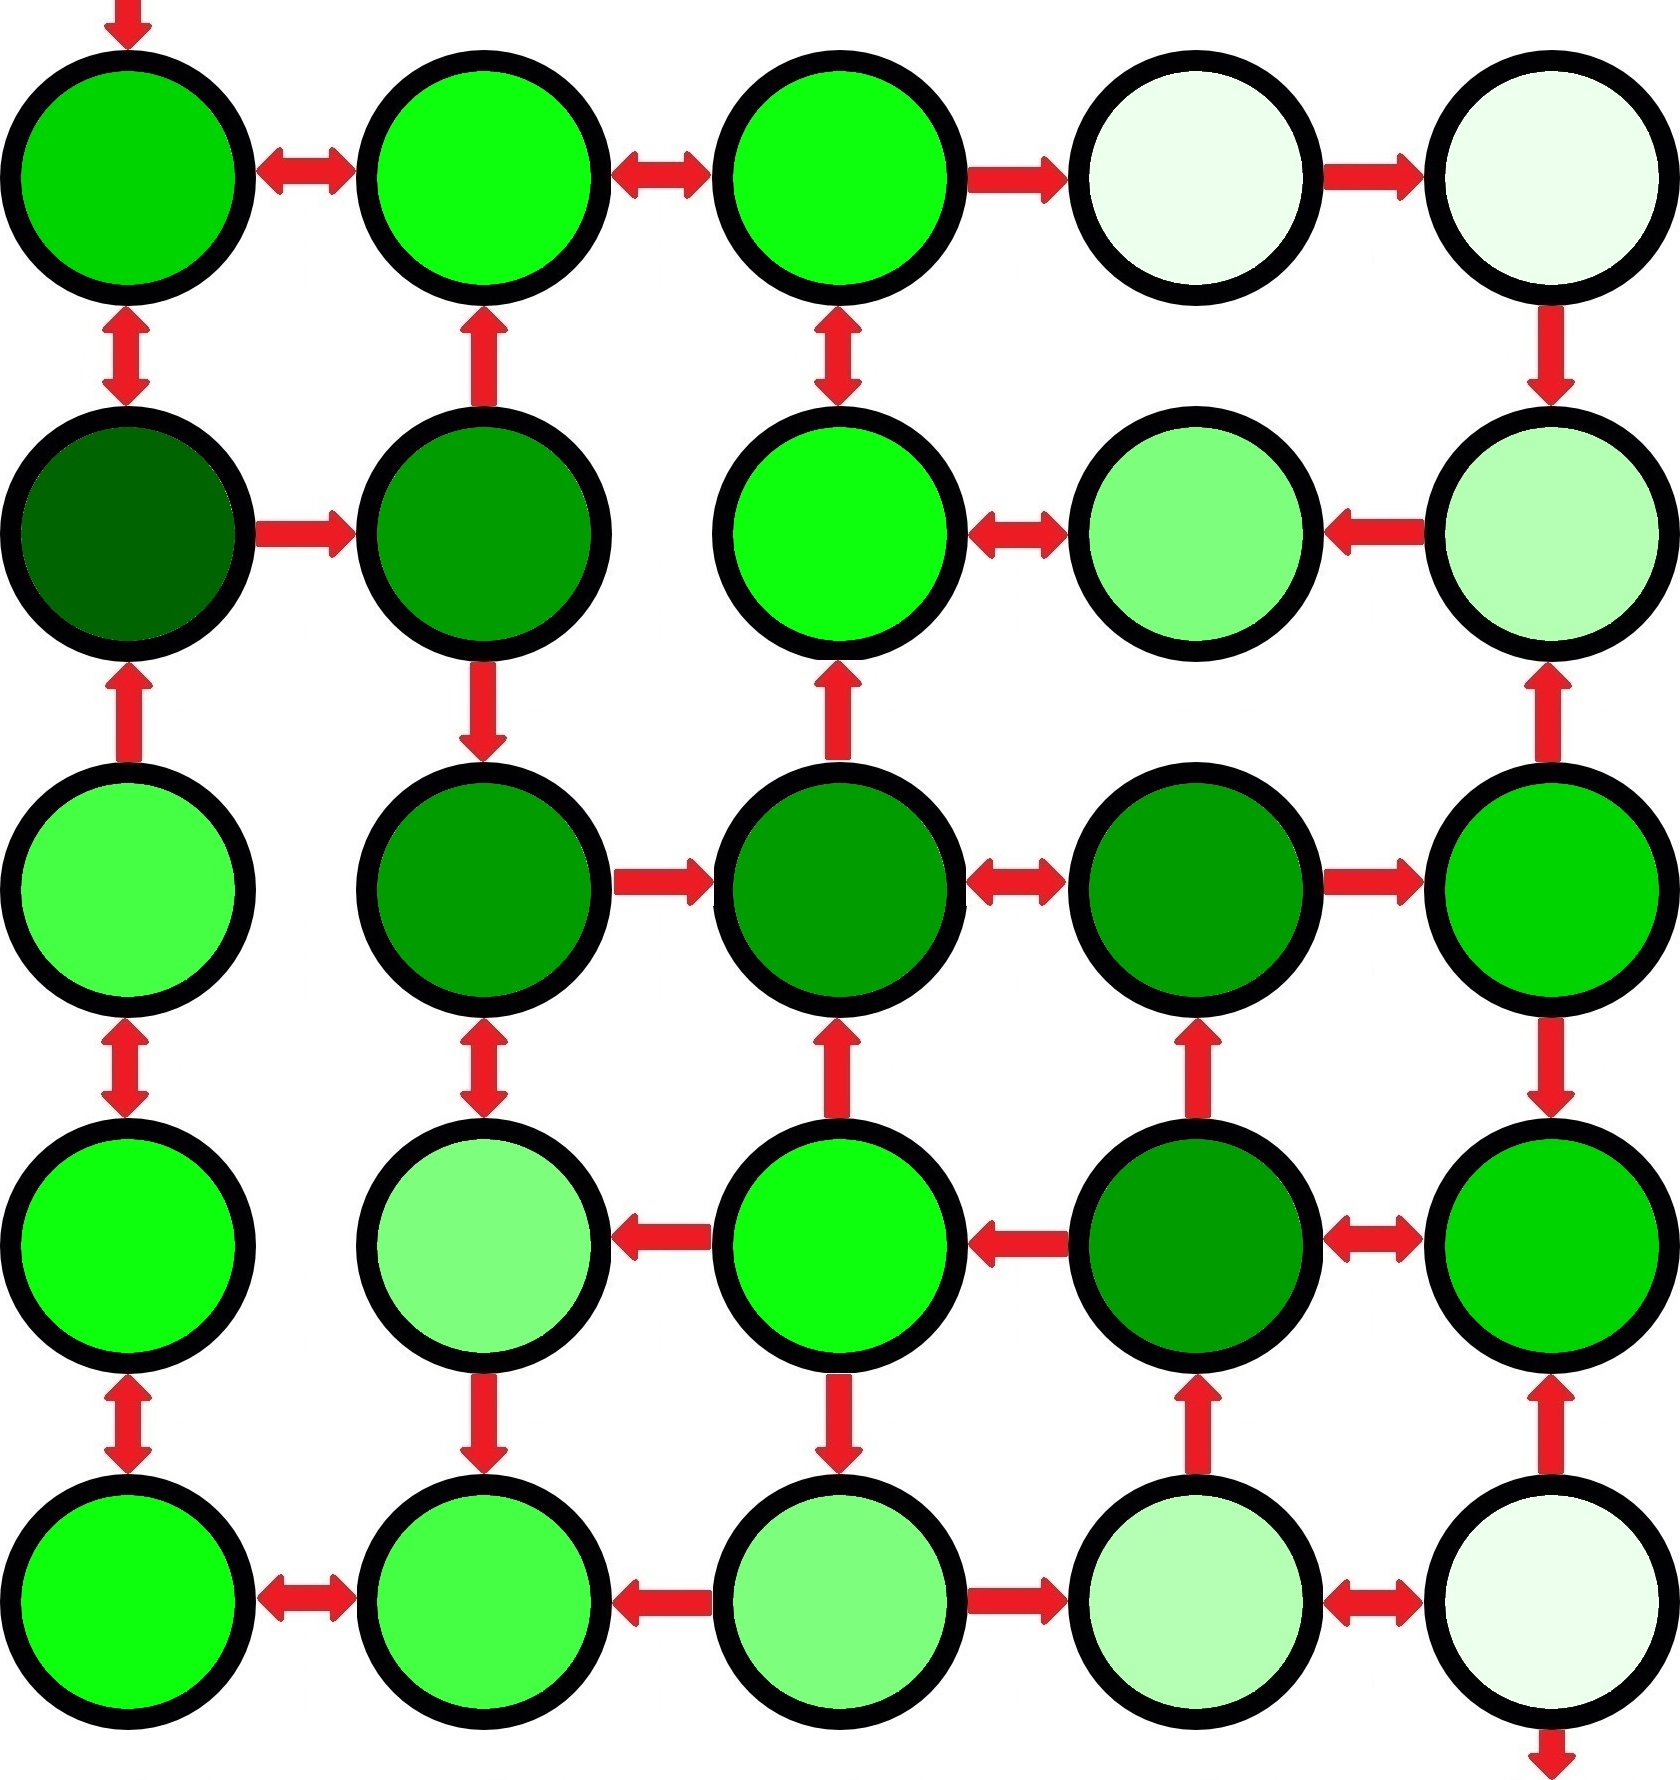
\includegraphics[width=1.0\textwidth]{Imagenes/Laberintos/25_calor.jpg}
	\caption{Mapa de calor del robot en el laberinto de 25 posiciones.}
	\label{fig:25_calor}
\end{figure}

\clearpage

\subsection{Análisis de los modelos}

Para lograr dar una respuesta sobre si es posible o no garantizar el cumplimiento del objetivo fue necesario 
explorar el entorno casi por completo. Las únicas dos acciones no ejecutadas fueron norte y oeste desde la posición 
final, por lo cual en el modelo del conocimiento van hacia \textit{La nube}.

\begin{figure}[H]
	\centering
		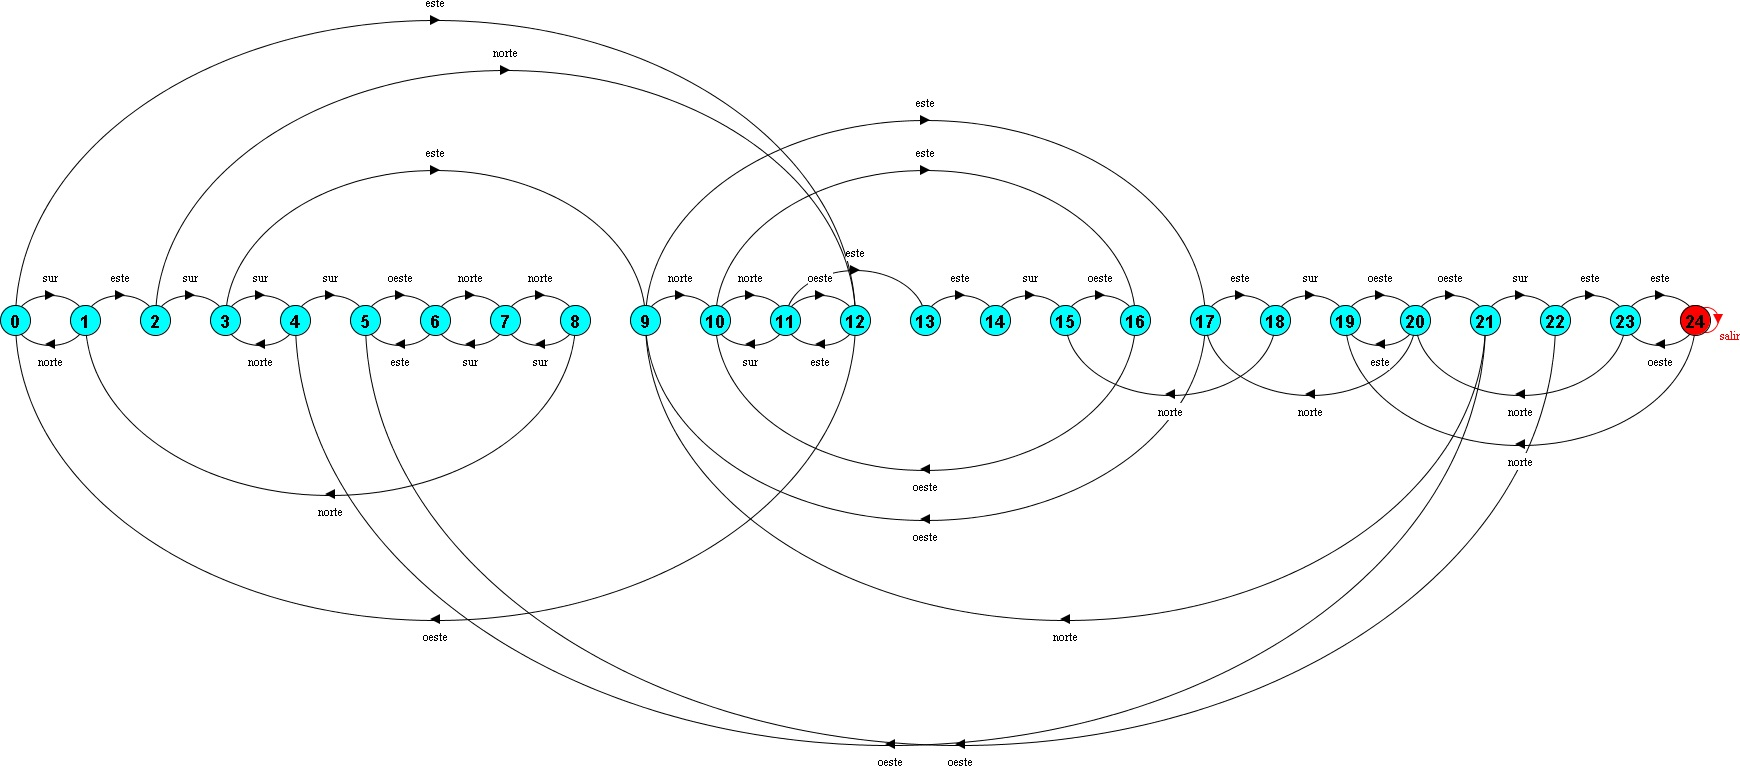
\includegraphics[width=1.0\textwidth]{Imagenes/Laberintos/25_view.jpg}
	\caption{LTS que representa al mapa del laberinto de 25 posiciones.}
	\label{fig:25_view}
\end{figure}

\begin{figure}[H]
	\centering
		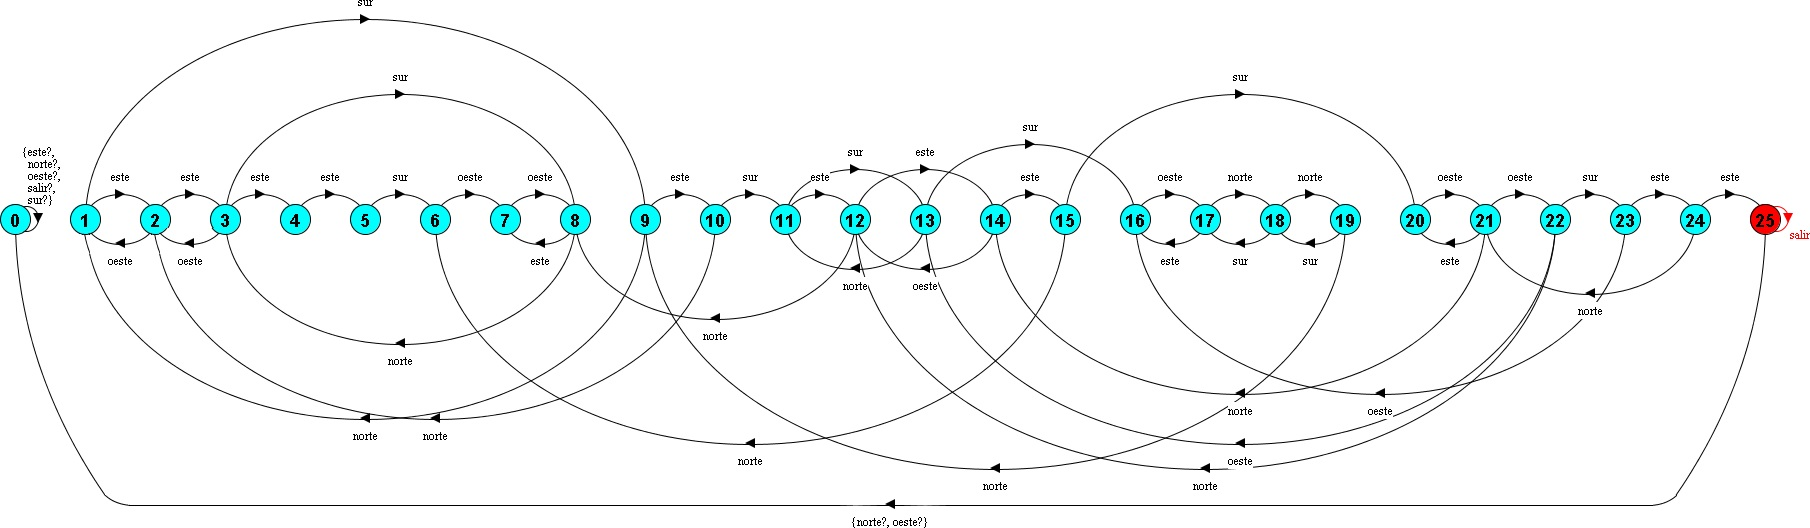
\includegraphics[width=1.0\textwidth]{Imagenes/Laberintos/25_knowledge.jpg}
	\caption{MTS que representa al conocimiento adquirido sobre el laberinto de 25 posiciones.}
	\label{fig:25_knowledge}
\end{figure}

\clearpage

\subsection{Variantes}

Si eliminamos la acción salir, el robot descubre que el laberinto no tiene salida en 122 pasos, formando un modelo 
de conocimiento de dos componentes conexas, en cual una componente conexa es bisimilar al LTS que representa al mapa, 
mientras que la otra componente conexa \textit{La nube}.

\vspace{\baselineskip}
Si modificamos el mapa para que la acción salir se encuentre en \textcolor[HTML]{0000A0}{P08} en vez de encontrarse 
en \textcolor[HTML]{0000A0}{P25}, el robot logra salir del laberinto en solamente 9 pasos, siendo su modelo del conocimiento 
mucho más reducido que el modelo del mapa.

\begin{figure}[H]
	\centering
		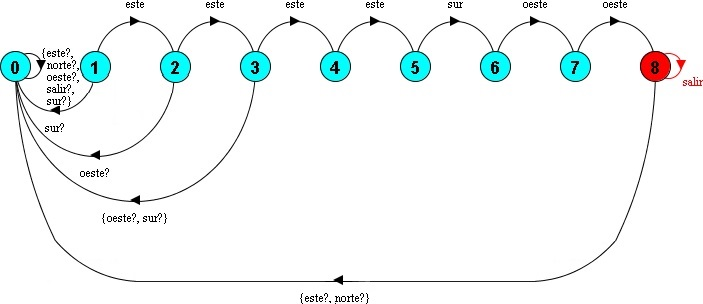
\includegraphics[width=1.0\textwidth]{Imagenes/Laberintos/25_knowledge_alternativo.jpg}
	\caption{MTS que representa al conocimiento adquirido sobre el laberinto de 25 posiciones con salida en la posición 8.}
	\label{fig:25_knowledge_alternativo}
\end{figure}

\clearpage

\section{Zonas inseguras}

En este ejemplo veremos como la estrategia Optimista utiliza nuestro conocimiento previo para evitar las zonas inseguras.

\begin{figure}[H]
	\centering
		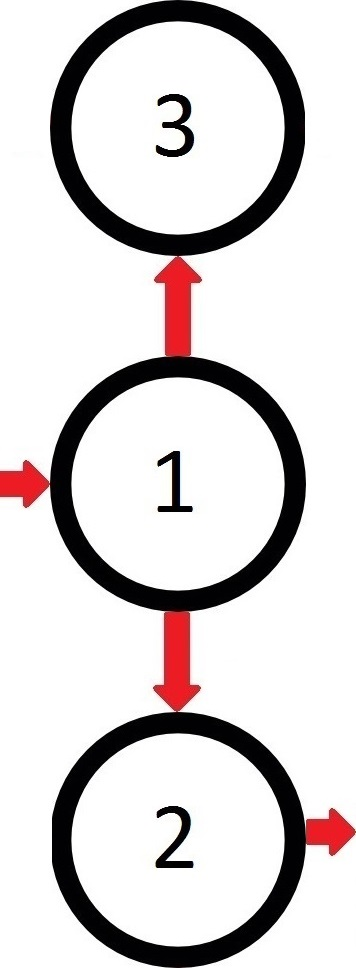
\includegraphics[width=0.15\textwidth]{Imagenes/Laberintos/unsafe.jpg}
	\caption{Laberinto con zona insegura.}
	\label{fig:unsafe}
\end{figure}

\subsection{Especificación en MTSA}

\begin{Code}[commandchars=&\[\]]
&fvtextcolor[0000A0][VIEW]   = (sur    -> &fvtextcolor[0000A0][GANAR] | norte -> &fvtextcolor[0000A0][PERDER]),
&fvtextcolor[0000A0][GANAR]  = (ganar  -> &fvtextcolor[0000A0][GANAR]),
&fvtextcolor[0000A0][PERDER] = (perder -> &fvtextcolor[0000A0][PERDER]).

&fvtextcolor[0000A0][MODEL_CON_INFO] = (sur?    -> &fvtextcolor[0000A0][MODEL_GANAR]    | norte?  -> &fvtextcolor[0000A0][MODEL_PERDER]  | 
                  ganar?  -> &fvtextcolor[0000A0][MODEL_CON_INFO] | perder? -> &fvtextcolor[0000A0][MODEL_CON_INFO]),
&fvtextcolor[0000A0][MODEL_GANAR]    = (sur?    -> &fvtextcolor[0000A0][MODEL_GANAR]    | norte?  -> &fvtextcolor[0000A0][MODEL_GANAR]   |
                  ganar?  -> &fvtextcolor[0000A0][MODEL_GANAR]),
&fvtextcolor[0000A0][MODEL_PERDER]   = (sur?    -> &fvtextcolor[0000A0][MODEL_PERDER]   | norte?  -> &fvtextcolor[0000A0][MODEL_PERDER]  | 
                  perder? -> &fvtextcolor[0000A0][MODEL_PERDER]).

&fvtextcolor[0000FF][set] &fvtextcolor[0000A0][Controllable_UNSAFE] = {norte, sur, ganar, perder}
&fvtextcolor[0000FF][fluent] &fvtextcolor[0000A0][F_Ganar]          = <ganar, &fvtextcolor[0000A0][Controllable_UNSAFE]\{ganar}>
&fvtextcolor[0000FF][assert] &fvtextcolor[0000A0][A_Ganar]          = &fvtextcolor[0000A0][F_Ganar]

&fvtextcolor[0000FF][controllerSpec] &fvtextcolor[0000A0][GOAL_UNSAFE] = {
    liveness     = {&fvtextcolor[0000A0][A_Ganar]}
    controllable = {&fvtextcolor[0000A0][Controllable_UNSAFE]}
}

&fvtextcolor[0000FF][exploration] &fvtextcolor[0000A0][UNSAFE] = {
    environment = {&fvtextcolor[0000A0][VIEW]},
    model       = {&fvtextcolor[0000A0][MODEL_CON_INFO]},
    goal        = {&fvtextcolor[0000A0][GOAL_UNSAFE]}
}
\end{Code}

\subsection{Análisis de los modelos}

\begin{figure}[H]
	\centering
		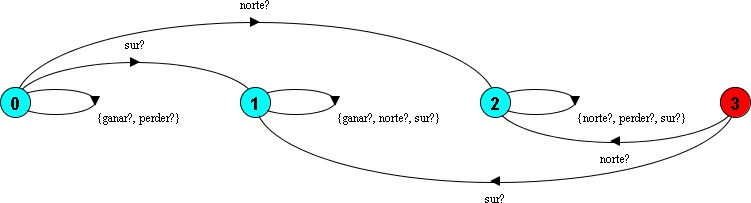
\includegraphics[width=1.0\textwidth]{Imagenes/Laberintos/unsafe_inicio.jpg}
	\caption{MTS que representa al conocimiento inicial sobre el laberinto con zona insegura.}
	\label{fig:unsafe_inicio}
\end{figure}

En la figura 4.7 podemos observar nuestro conocimiento sobre el entorno al iniciar la exploración. Los estados 0, 1 y 2 pertenecen a \textit{La nube}, 
el estado 3 es el estado inicial.

\begin{figure}[H]
	\centering
		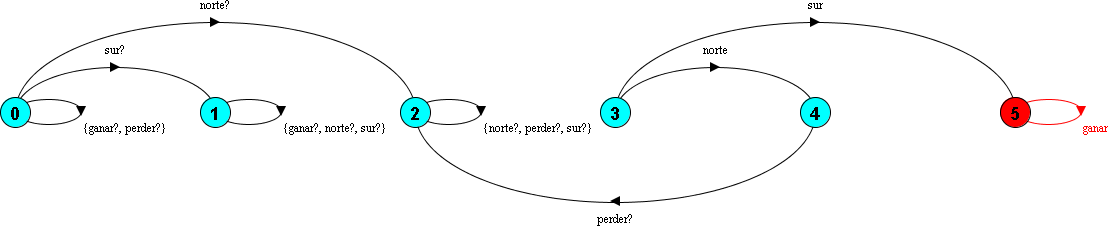
\includegraphics[width=1.0\textwidth]{Imagenes/Laberintos/unsafe_nueva_accion.png}
	\caption{MTS que representa al conocimiento adquirido sobre el laberinto con zona insegura, utilizando la estrategia Nueva Acción.}
	\label{fig:unsafe_nueva_accion}
\end{figure}

Si utilizamos la estrategia Nueva Acción, lo único que importa es elegir una acción nueva. En el caso de la figura 4.8, la estrategia eligió primero norte, 
llegando así a un estado sin salida. Fue necesario realizar un reset para luego elegir sur y llegar a un estado ganador.

\begin{figure}[H]
	\centering
		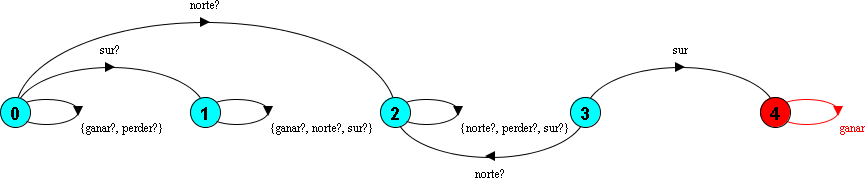
\includegraphics[width=1.0\textwidth]{Imagenes/Laberintos/unsafe_sintesis.png}
	\caption{MTS que representa al conocimiento adquirido sobre el laberinto con zona insegura, utilizando la estrategia Optimista - Nueva Acción.}
	\label{fig:unsafe_sintesis}
\end{figure}

En cambio, utilizando la estrategia Optimista - Nueva Acción, por construcción, el controlador optimista evita las zonas inseguras. Al elegir la acción, 
se descarta norte, por lo cual el robot llega a un estado ganador sin la necesidad de realizar un reset, como puede observarse en la figura 4.9.

\clearpage

\section{Laberinto que baja}

En este ejemplo, el robot se puede mover libremente en forma horizontal, ya que si se mueve a izquierda o derecha, siempre puede regresar a la posición en la que estaba. 
Si el robot se mueve hacia abajo no puede volver a subir. La salida no se encuentra en el nivel inferior, por lo cual todos los estados del nivel inferior son estados perdedores.

\begin{figure}[H]
	\centering
		\includegraphics[width=1.0\textwidth]{Imagenes/Laberintos/down.jpg}
	\caption{Laberinto que baja.}
	\label{fig:down}
\end{figure}

\subsection{Especificación en MTSA}

\begin{Code}[commandchars=&\[\]]
&fvtextcolor[0000A0][VIEW] = &fvtextcolor[0000A0][P03],
&fvtextcolor[0000A0][P01] = (este  -> &fvtextcolor[0000A0][P02]),
&fvtextcolor[0000A0][P02] = (sur   -> &fvtextcolor[0000A0][P07] | este  -> &fvtextcolor[0000A0][P03] | oeste -> &fvtextcolor[0000A0][P01]),
&fvtextcolor[0000A0][P03] = (este  -> &fvtextcolor[0000A0][P04] | oeste -> &fvtextcolor[0000A0][P02]),
&fvtextcolor[0000A0][P04] = (este  -> &fvtextcolor[0000A0][P05] | oeste -> &fvtextcolor[0000A0][P03]),
&fvtextcolor[0000A0][P05] = (sur   -> &fvtextcolor[0000A0][P10] | oeste -> &fvtextcolor[0000A0][P04]),
&fvtextcolor[0000A0][P06] = (este  -> &fvtextcolor[0000A0][P07]),
&fvtextcolor[0000A0][P07] = (este  -> &fvtextcolor[0000A0][P08] | oeste -> &fvtextcolor[0000A0][P06]),
&fvtextcolor[0000A0][P08] = (sur   -> &fvtextcolor[0000A0][P13] | oeste -> &fvtextcolor[0000A0][P07]),
&fvtextcolor[0000A0][P09] = (este  -> &fvtextcolor[0000A0][P10]),
&fvtextcolor[0000A0][P10] = (sur   -> &fvtextcolor[0000A0][P15] | oeste -> &fvtextcolor[0000A0][P09]),
&fvtextcolor[0000A0][P11] = (este  -> &fvtextcolor[0000A0][P12] | salir -> &fvtextcolor[0000A0][P11]),
&fvtextcolor[0000A0][P12] = (sur   -> &fvtextcolor[0000A0][P17] | este  -> &fvtextcolor[0000A0][P13] | oeste -> &fvtextcolor[0000A0][P11]),
&fvtextcolor[0000A0][P13] = (sur   -> &fvtextcolor[0000A0][P18] | este  -> &fvtextcolor[0000A0][P14] | oeste -> &fvtextcolor[0000A0][P12]),
&fvtextcolor[0000A0][P14] = (sur   -> &fvtextcolor[0000A0][P19] | este  -> &fvtextcolor[0000A0][P15] | oeste -> &fvtextcolor[0000A0][P13]),
&fvtextcolor[0000A0][P15] = (sur   -> &fvtextcolor[0000A0][P20] | oeste -> &fvtextcolor[0000A0][P14]),
&fvtextcolor[0000A0][P16] = (este  -> &fvtextcolor[0000A0][P17]),
&fvtextcolor[0000A0][P17] = (oeste -> &fvtextcolor[0000A0][P16]),
&fvtextcolor[0000A0][P18] = (este  -> &fvtextcolor[0000A0][P19]),
&fvtextcolor[0000A0][P19] = (este  -> &fvtextcolor[0000A0][P20] | oeste -> &fvtextcolor[0000A0][P18]),
&fvtextcolor[0000A0][P20] = (oeste -> &fvtextcolor[0000A0][P19]).

&fvtextcolor[0000A0][MODEL_CON_INFO] = &fvtextcolor[0000A0][CENTRO],
&fvtextcolor[0000A0][CENTRO]  = (sur?   -> &fvtextcolor[0000A0][CENTRO]  | este?  -> &fvtextcolor[0000A0][ESTE_1] | 
           oeste? -> &fvtextcolor[0000A0][OESTE_1] | salir? -> &fvtextcolor[0000A0][CENTRO]),
&fvtextcolor[0000A0][ESTE_1]  = (sur?   -> &fvtextcolor[0000A0][CENTRO]  | este?  -> &fvtextcolor[0000A0][ESTE_2] | 
           oeste  -> &fvtextcolor[0000A0][CENTRO]  | salir? -> &fvtextcolor[0000A0][ESTE_1]),
&fvtextcolor[0000A0][ESTE_2]  = (sur?   -> &fvtextcolor[0000A0][CENTRO]  | este?  -> &fvtextcolor[0000A0][ESTE_3] | 
           oeste  -> &fvtextcolor[0000A0][ESTE_1]  | salir? -> &fvtextcolor[0000A0][ESTE_2]),
&fvtextcolor[0000A0][ESTE_3]  = (sur?   -> &fvtextcolor[0000A0][CENTRO]  | este?  -> &fvtextcolor[0000A0][ESTE_4] | 
           oeste  -> &fvtextcolor[0000A0][ESTE_2]  | salir? -> &fvtextcolor[0000A0][ESTE_3]),
&fvtextcolor[0000A0][ESTE_4]  = (sur?   -> &fvtextcolor[0000A0][CENTRO]  | oeste  -> &fvtextcolor[0000A0][ESTE_3] | 
           salir? -> &fvtextcolor[0000A0][ESTE_4]),
&fvtextcolor[0000A0][OESTE_1] = (sur?   -> &fvtextcolor[0000A0][CENTRO]  | este   -> &fvtextcolor[0000A0][CENTRO]  | 
           oeste? -> &fvtextcolor[0000A0][OESTE_2] | salir? -> &fvtextcolor[0000A0][OESTE_1]),
&fvtextcolor[0000A0][OESTE_2] = (sur?   -> &fvtextcolor[0000A0][CENTRO]  | este   -> &fvtextcolor[0000A0][OESTE_1] | 
           oeste? -> &fvtextcolor[0000A0][OESTE_3] | salir? -> &fvtextcolor[0000A0][OESTE_2]),
&fvtextcolor[0000A0][OESTE_3] = (sur?   -> &fvtextcolor[0000A0][CENTRO]  | este   -> &fvtextcolor[0000A0][OESTE_2] | 
           oeste? -> &fvtextcolor[0000A0][OESTE_4] | salir? -> &fvtextcolor[0000A0][OESTE_3]),
&fvtextcolor[0000A0][OESTE_4] = (sur?   -> &fvtextcolor[0000A0][CENTRO]  | este   -> &fvtextcolor[0000A0][OESTE_3] | 
           salir? -> &fvtextcolor[0000A0][OESTE_4]).

&fvtextcolor[0000FF][set] &fvtextcolor[0000A0][Controllable_Down] = {sur, este, oeste, salir}
&fvtextcolor[0000FF][fluent] &fvtextcolor[0000A0][F_Salir]        = <salir, &fvtextcolor[0000A0][Controllable_Down]\{salir}>
&fvtextcolor[0000FF][assert] &fvtextcolor[0000A0][A_Salir]        = &fvtextcolor[0000A0][F_Salir]

&fvtextcolor[0000FF][controllerSpec] &fvtextcolor[0000A0][GOAL_Down] = {
    liveness     = {&fvtextcolor[0000A0][A_Salir]}
    controllable = {&fvtextcolor[0000A0][Controllable_Down]}
}

&fvtextcolor[0000FF][exploration] &fvtextcolor[0000A0][MDown] = {
    environment = {&fvtextcolor[0000A0][VIEW]},
    model       = {&fvtextcolor[0000A0][MODEL_CON_INFO]},
    goal        = {&fvtextcolor[0000A0][GOAL_Down]}
}
\end{Code}

\clearpage

\subsection{Análisis de los modelos}

Sabemos que:
\begin{itemize}

\item
Si podemos movernos una posición horizontalmente, también vamos a poder movernos una posición en la dirección contraria.

\item
Como máximo podemos movernos hasta cuatro veces en la misma dirección.

\item
Si bajamos, llegamos a una posición que cumple las dos condiciones antes mencionadas.

\end{itemize}

Vamos a utilizar como modelo del conocimiento inicial un MTS que represente estas tres condiciones.

\begin{figure}[H]
	\centering
		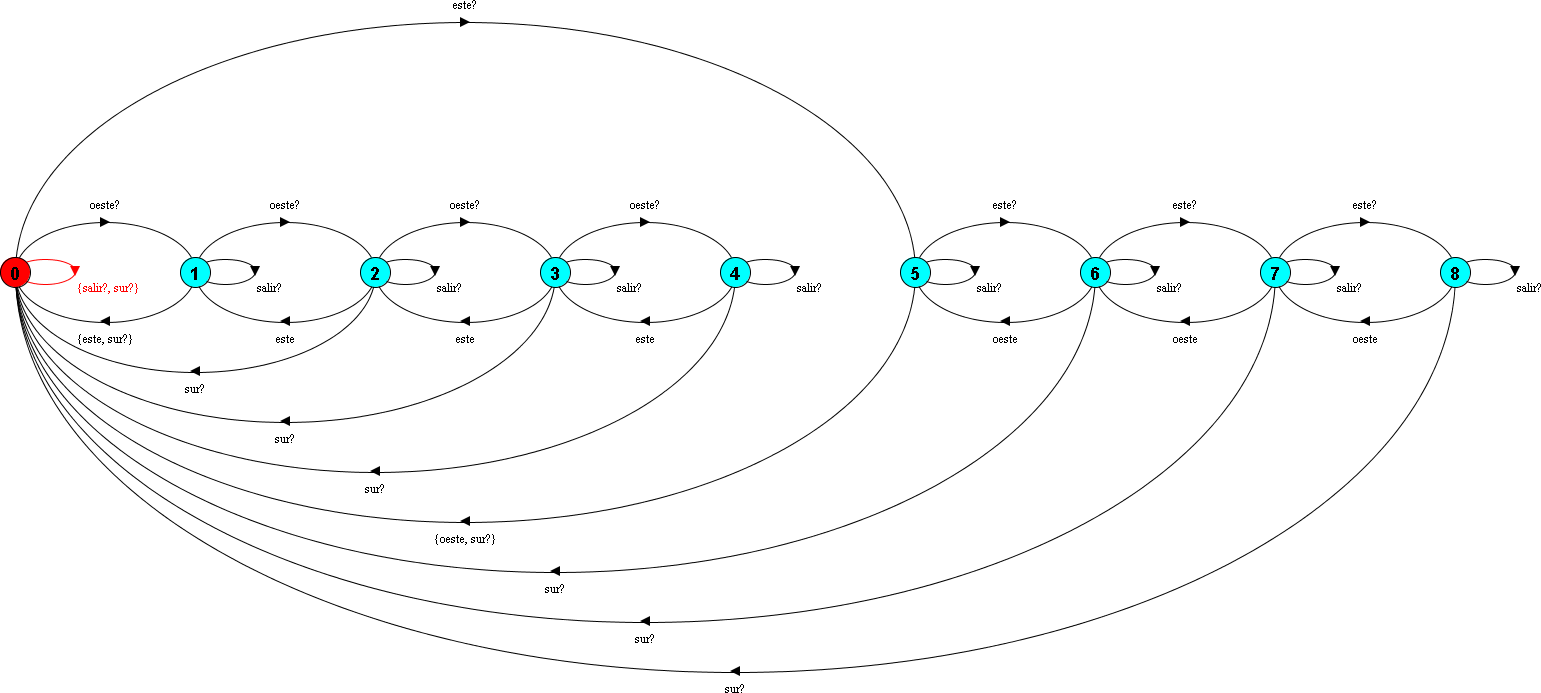
\includegraphics[width=1.0\textwidth]{Imagenes/Laberintos/down_modelo.png}
	\caption{MTS que representa al conocimiento inicial sobre el laberinto que baja.}
	\label{fig:down_modelo}
\end{figure}

El problema está en que no podemos modelar la siguiente condición:
\begin{itemize}
\item
Si podemos movernos una posición horizontalmente, también vamos a poder movernos a \textbf{la misma} posición de la que partimos.
\end{itemize}

Por carecer de esta condición, no podemos saber que las acciones de movimiento horizontal son más seguras que la acción bajar, 
ya que la acción bajar nos puede llevar a un estado perdedor desde un estado ganador, cosa que no puede pasar con las acciones horizontales.

\clearpage

\subsection{Resultado}

\begin{figure}[H]
	\centering
		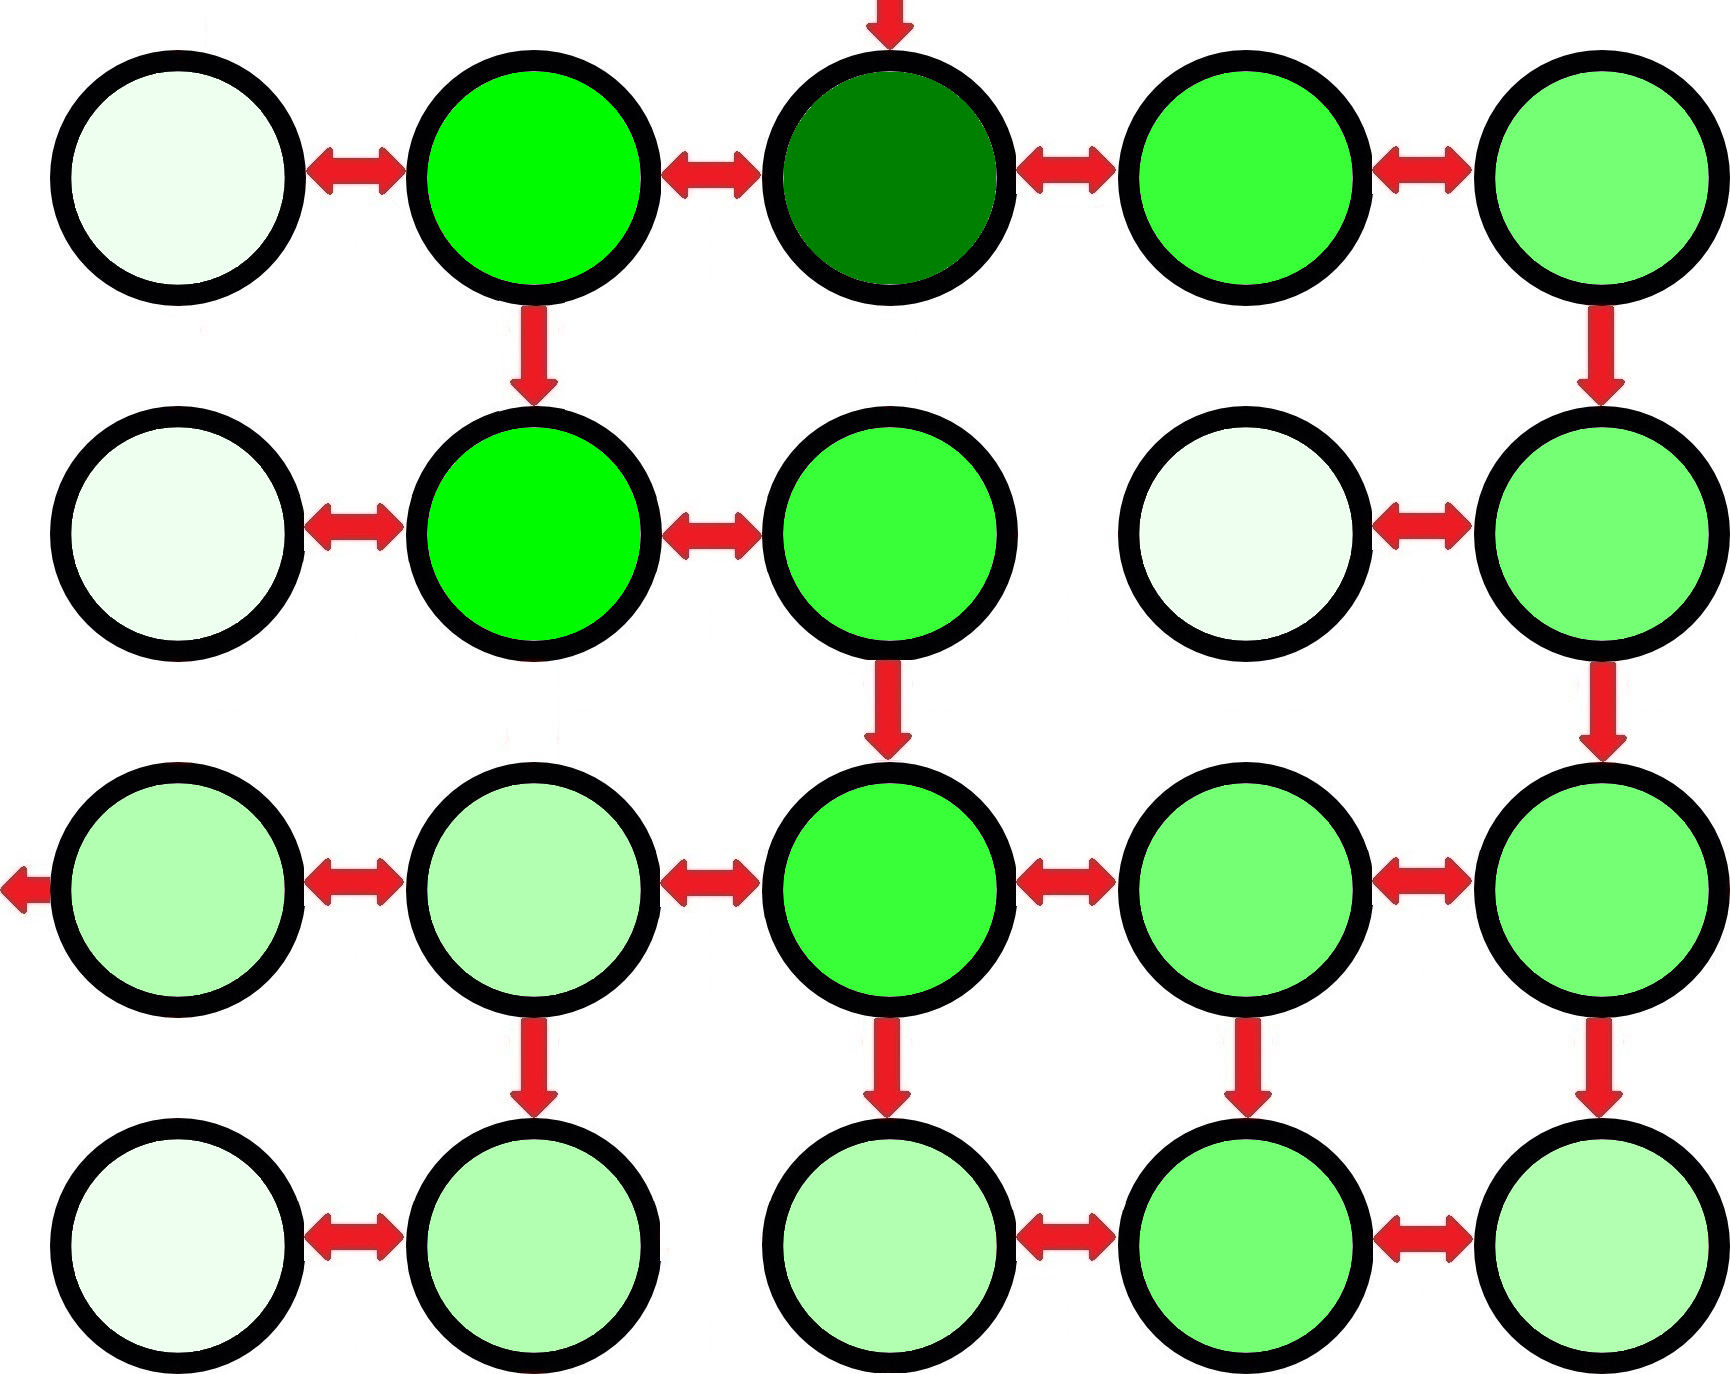
\includegraphics[width=1.0\textwidth]{Imagenes/Laberintos/down_calor.png}
	\caption{Mapa de calor del robot en el laberinto que baja.}
	\label{fig:down_calor}
\end{figure}

El robot logra salir del laberinto en 58 pasos, para lo cual fue necesario realizar un reset en 4 oportunidades. 
Al no poder distinguir los estados seguros de los que nos pueden llevar a estados perdedores, la estrategia elige arbitrariamente 
cualquier acción nueva, cayendo varias veces en estados perdedores.

\clearpage

\section{Laberinto con puente}

En este ejemplo, el robot puede moverse libremente entre todas las posiciones contiguas, pero entre las posiciones 7 y 8 hay un puente 
controlado por un agente externo, quien puede cerrar el paso.

\begin{figure}[H]
	\centering
		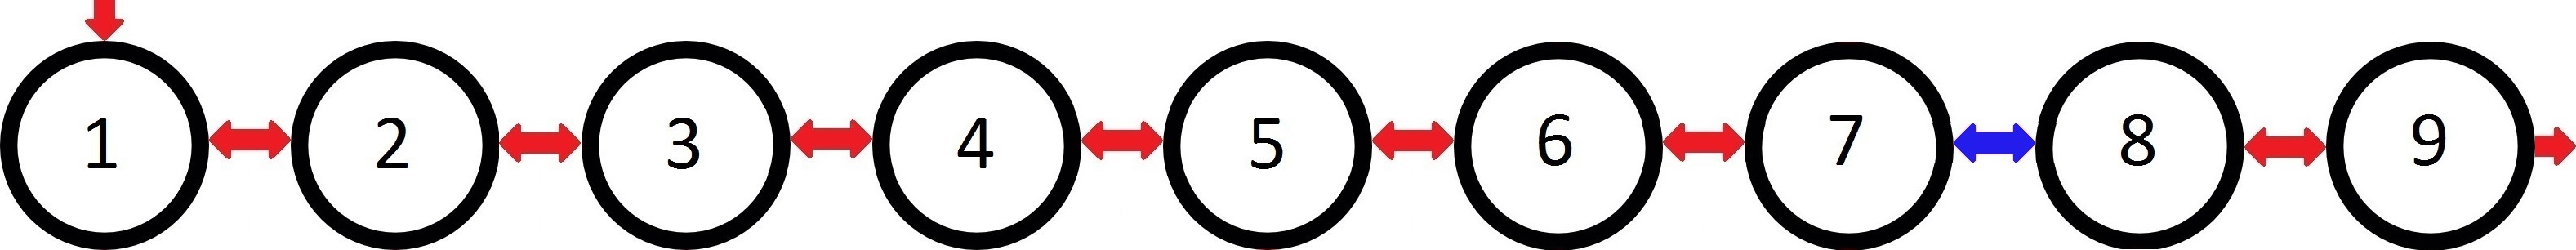
\includegraphics[width=1.0\textwidth]{Imagenes/Laberintos/puente.jpg}
	\caption{Laberinto con puente.}
	\label{fig:puente}
\end{figure}

Este ejemplo introduce un agente externo, por lo cual vamos a necesitar definir:

\begin{itemize}

\item
Un LTS que represente el comportamiento del agente externo. Indica que acciones puede realizar el agente externo en cada momento.

\item
Un MTS que represente nuestro conocimiento inicial sobre el comportamiento del agente externo. 
El robot adquirirá conocimiento sobre el agente externo a medida que pueda observar sus acciones.

\item
Una suposición de dominio sobre el comportamiento del agente externo, la cual garantice que el agente externo no va a impedir 
que alcancemos nuestro objetivo.

\item
Aunque es opcional, vamos a utilizar una lista de acciones que ejecutará el agente externo cíclicamente. 
De esta forma, especificamos su comportamiento para este ejemplo.

En caso de que hubiera más de un agente externo, deberíamos definir estos cuatro items para cada uno de ellos.

\end{itemize}

\clearpage

\subsection{Especificación en MTSA}

\begin{Code}[commandchars=&\[\]]
&fvtextcolor[0000A0][MAPA] = &fvtextcolor[0000A0][M1],
&fvtextcolor[0000A0][M1] = (este   -> &fvtextcolor[0000A0][M2]),
&fvtextcolor[0000A0][M2] = (este   -> &fvtextcolor[0000A0][M3] | oeste  -> &fvtextcolor[0000A0][M1]),
&fvtextcolor[0000A0][M3] = (este   -> &fvtextcolor[0000A0][M4] | oeste  -> &fvtextcolor[0000A0][M2]),
&fvtextcolor[0000A0][M4] = (este   -> &fvtextcolor[0000A0][M5] | oeste  -> &fvtextcolor[0000A0][M3]),
&fvtextcolor[0000A0][M5] = (este   -> &fvtextcolor[0000A0][M6] | oeste  -> &fvtextcolor[0000A0][M4]),
&fvtextcolor[0000A0][M6] = (este   -> &fvtextcolor[0000A0][M7] | oeste  -> &fvtextcolor[0000A0][M5]),
&fvtextcolor[0000A0][M7] = (cruzar -> &fvtextcolor[0000A0][M8] | oeste  -> &fvtextcolor[0000A0][M6]),
&fvtextcolor[0000A0][M8] = (este   -> &fvtextcolor[0000A0][M9] | cruzar -> &fvtextcolor[0000A0][M7]),
&fvtextcolor[0000A0][M9] = (oeste  -> &fvtextcolor[0000A0][M8] | ganar  -> &fvtextcolor[0000A0][M9]).

&fvtextcolor[0000A0][PUENTE] = &fvtextcolor[0000A0][PUENTE_CERRADO],
&fvtextcolor[0000A0][PUENTE_CERRADO] = (abrir  -> &fvtextcolor[0000A0][PUENTE_ABIERTO] | cerrar -> &fvtextcolor[0000A0][PUENTE_CERRADO]),
&fvtextcolor[0000A0][PUENTE_ABIERTO] = (abrir  -> &fvtextcolor[0000A0][PUENTE_ABIERTO] | cruzar -> &fvtextcolor[0000A0][PUENTE_ABIERTO] | 
                  cerrar -> &fvtextcolor[0000A0][PUENTE_CERRADO]).

&fvtextcolor[0000A0][MTS_MAPA]   = (este?   -> &fvtextcolor[0000A0][MTS_MAPA]   | oeste?  -> &fvtextcolor[0000A0][MTS_MAPA]   | 
              cruzar? -> &fvtextcolor[0000A0][MTS_MAPA]   | ganar?  -> &fvtextcolor[0000A0][MTS_MAPA]).
							
&fvtextcolor[0000A0][MTS_PUENTE] = (abrir?  -> &fvtextcolor[0000A0][MTS_PUENTE] | cerrar? -> &fvtextcolor[0000A0][MTS_PUENTE] | 
              cruzar? -> &fvtextcolor[0000A0][MTS_PUENTE]).

&fvtextcolor[0000FF][set] &fvtextcolor[0000A0][Controllable_puente] = {este, oeste, cruzar, ganar}

&fvtextcolor[0000FF][fluent] &fvtextcolor[0000A0][F_Ganar] = <ganar, &fvtextcolor[0000A0][Controllable_puente]\{ganar}>
&fvtextcolor[0000FF][assert] &fvtextcolor[0000A0][A_Ganar] = &fvtextcolor[0000A0][F_Ganar]

&fvtextcolor[0000FF][fluent] &fvtextcolor[0000A0][F_PuedeCruzar] = <abrir, cruzar>
&fvtextcolor[0000FF][assert] &fvtextcolor[0000A0][PuedeCruzar]   = &fvtextcolor[0000A0][F_PuedeCruzar]

&fvtextcolor[0000FF][controllerSpec] &fvtextcolor[0000A0][GOAL_PUENTE] = {
    assumption   = {&fvtextcolor[0000A0][PuedeCruzar]}
    liveness     = {&fvtextcolor[0000A0][A_Ganar]}
    controllable = {&fvtextcolor[0000A0][Controllable_puente]}
}

&fvtextcolor[0000FF][exploration] &fvtextcolor[0000A0][PUENTE_CON_SALIDA] = {
    environment         = {&fvtextcolor[0000A0][MAPA], &fvtextcolor[0000A0][PUENTE]},
    model               = {&fvtextcolor[0000A0][MTS_MAPA], &fvtextcolor[0000A0][MTS_PUENTE]},
    goal                = {&fvtextcolor[0000A0][GOAL_PUENTE]},
    environment_actions = {{cerrar, cerrar, cerrar, cerrar, cerrar,
                            cerrar, cerrar, cerrar, cerrar, cerrar, 
                            abrir, abrir, abrir}}
}
\end{Code}

\clearpage

\subsection{Análisis de los modelos}

Como el robot observa todas las acciones del agente externo, al final de la exploración, el MTS que representa su comportamiento está completamente refinado.

\begin{figure}[H]
	\centering
		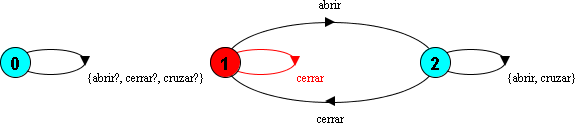
\includegraphics[width=1.0\textwidth]{Imagenes/Laberintos/puente_modelo_puente.png}
	\caption{MTS que representa al conocimiento adquirido sobre el agente externo del laberinto con puente.}
	\label{fig:puente_modelo_puente}
\end{figure}

En cuanto al mapa, la única acción no ejecutada es cruzar desde el estado 8 al estado 7.

\begin{figure}[H]
	\centering
		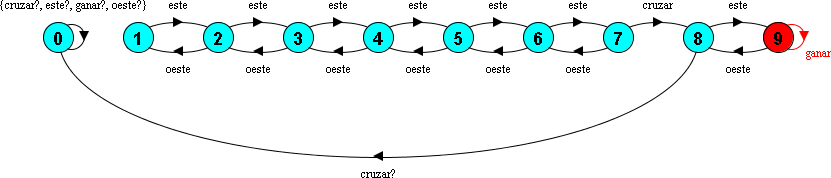
\includegraphics[width=1.0\textwidth]{Imagenes/Laberintos/puente_modelo_mapa.png}
	\caption{MTS que representa al conocimiento adquirido sobre el laberinto con puente.}
	\label{fig:puente_modelo_mapa}
\end{figure}

\subsection{Análisis de la traza}

El robot logra salir del laberinto en 30 pasos. Podemos observar que cuando el robot termina de explorar completamente los estados 1 a 7, 
va hasta el estado 7 a esperar que el agente externo abra el puente, en vez de esperarlo en su estado actual, ya que solamente desde el estado 7 
puede beneficiarse de las acciones del agente externo.

\vspace{\baselineskip}

El robot sabe que el agente externo va a abrir el puente por la suposición de dominio que tenemos. En caso de no tener esta suposición, 
en vez de esperar, el robot asumiría que no se puede garantizar el cumplimiento del objetivo, ya que el agente externo podría no abrir el puente nunca.

\begin{figure}[H]
	\centering
		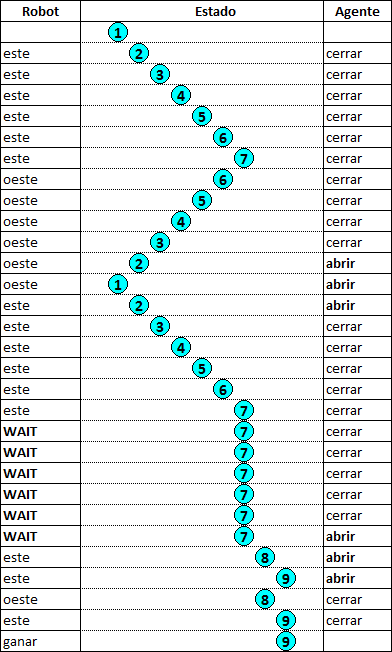
\includegraphics[width=0.8\textwidth]{Imagenes/Laberintos/puente_traza.png}
	\caption{Traza del robot en el laberinto con puente.}
	\label{fig:puente_traza}
\end{figure}
